% Created 2024-09-03 Tue 08:34
% Intended LaTeX compiler: pdflatex
\documentclass[letterpaper, 12pt]{article}
\usepackage[utf8]{inputenc}
\usepackage[T1]{fontenc}
\usepackage{graphicx}
\usepackage{longtable}
\usepackage{wrapfig}
\usepackage{rotating}
\usepackage[normalem]{ulem}
\usepackage{amsmath}
\usepackage{amssymb}
\usepackage{capt-of}
\usepackage{hyperref}
\usepackage{minted}
\usepackage{xcolor}
\usepackage{hyperref}
\usepackage{tocloft}
\usepackage{minted}
\usemintedstyle{manni}
\usepackage{pdfpages}
\usepackage{fancyhdr}
\usepackage{graphicx}
\usepackage[top=1.4in, left=0.5in, right=0.5in, bottom=0.8in]{geometry}
\usepackage[T1]{fontenc}
\usepackage{helvet}
\pagestyle{fancy}
\renewcommand{\headrulewidth}{0pt}
\renewcommand{\footrulewidth}{0pt}
\setlength{\parindent}{0em}
\setlength{\parskip}{1em}
\usepackage{hyperref}
\usepackage {color}
\usepackage {tabularray}
\usepackage{xcolor}
\hypersetup{
colorlinks=true,
linkcolor=blue,
filecolor=magenta,
urlcolor=cyan,
citecolor=green,
pdfborder={0 0 0}
}
\usepackage[most]{tcolorbox}
\author{School Administration Hilduara Abreu}
\date{2024-09-05}
\title{PS 192 | Responding to Door Alarm Protocol}
\hypersetup{
 pdfauthor={School Administration Hilduara Abreu},
 pdftitle={PS 192 | Responding to Door Alarm Protocol},
 pdfkeywords={},
 pdfsubject={},
 pdfcreator={Emacs 29.4 (Org mode 9.6.15)}, 
 pdflang={English}}
\begin{document}

\fancyfoot[C]{\setlength{\unitlength}{1in}\begin{picture}(5,0)\put(-1.8,-0.5){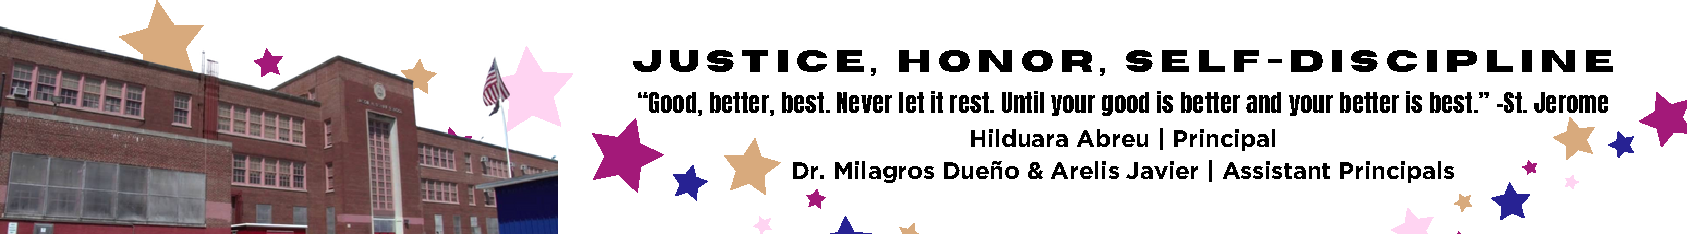
\includegraphics[width=8.8in,height=1.3in]{logo-1}}\end{picture}}
\fancyhead[C]{\setlength{\unitlength}{1in}\begin{picture}(5,0)\put(-1.9,-0.5){
\includegraphics[width=8.9in,height=1.3in]{logo-2}}\end{picture}}
\fancyhead[R]{\thepage}
\pagenumbering{gobble}

\begin{document}
\newpage
\vspace*{-0.5cm}
\textbf{PS 192 | Responding to Door Alarm Protocol}

\textbf{Objective}

To ensure the safety and security of all students, staff, and visitors at PS 192 by providing clear guidelines for responding to door alarms in compliance with NYC DOE regulations.

\textbf{Purpose}

The purpose of this protocol is to outline the steps that must be taken immediately when a door alarm is activated within the school premises. This protocol is designed to ensure a prompt, effective, and coordinated response to any potential security breach or unauthorized exit.

\textbf{Immediate Response}
\begin{itemize}
\item Assess the Situation
\begin{itemize}
\item Upon hearing a door alarm, the nearest staff member must immediately assess the situation.
\item Determine whether the alarm was triggered accidentally or if it indicates an unauthorized exit or security breach.
\end{itemize}
\item Report the Alarm
\begin{itemize}
\item The staff member who responds to the alarm must immediately notify the School Safety Agent (SSA) and a member of the Admin Team.
\item Provide the exact location of the alarm and any observations regarding the situation (e.g., students nearby, open doors, etc.).
\end{itemize}
\end{itemize}

\textbf{Security Check}
\begin{itemize}
\item School Safety Agent (SSA) Response
\begin{itemize}
\item The School Safety Agent (SSA) or designated security personnel must proceed to the location of the alarm immediately.
\item Conduct a thorough check of the area to ensure that there is no unauthorized exit or entry.
\item If the door has been breached, the SSA must secure the area and take note of any suspicious activity or individuals.
\end{itemize}
\end{itemize}

\textbf{Classroom and Hallway Check}
\newpage \vspace*{-0.5cm}
\begin{itemize}
\item Teachers in nearby classrooms must conduct a quick headcount to ensure that all students are accounted for.
\item Any unaccounted students must be reported to a member of the admin team via text immediately.
\end{itemize}

\textbf{Communication and Coordination}
\begin{itemize}
\item Intercom Announcement
\begin{itemize}
\item The secretary will make a brief intercom announcement to inform the school community that a door alarm has been activated and that the situation is being addressed.
\item Example Announcement: "Attention, staff and students: A door alarm has been triggered. Please remain in your current locations while the situation is being investigated."
\end{itemize}
\end{itemize}

\textbf{Administration Notification}
\begin{itemize}
\item The administration will coordinate with the SSA to determine whether additional measures are required, such as a lockdown or notifying law enforcement.
\end{itemize}

\textbf{Investigation and Documentation}
\begin{itemize}
\item Identify the Cause
\begin{itemize}
\item The SSA, in collaboration with the administration, will investigate the cause of the alarm.
\item If it is determined that the alarm was triggered accidentally (e.g., by a student or staff member).
\end{itemize}
\end{itemize}

\textbf{Unauthorized Exit}
\begin{itemize}
\item If the alarm indicates an unauthorized exit (e.g., a student leaving the building without permission), the administration will take immediate action to locate the student (per the Missing Student Protocol).
\item Parents/guardians will be notified as soon as possible, and appropriate disciplinary measures will be taken in accordance with NYC DOE regulations.
\end{itemize}

\textbf{Incident Documentation}
\newpage \vspace*{-0.5cm}
\begin{itemize}
\item The incident must be documented using the Online Occurrence Reporting System (OORS) by the end of the school day by Dr. Dueno.
\item The report should include details of the incident, the response actions taken, and any follow-up measures required.
\end{itemize}

\textbf{Preventive Measures}
\begin{itemize}
\item Regular Alarm Testing
\begin{itemize}
\item Alarms will be tested regularly to ensure they are functioning correctly.
\item Any malfunctions or issues with the alarm system will be reported immediately to the DSF, Custodian, and D6 Superintendent for repair.
\end{itemize}
\end{itemize}

\textbf{Doors and Alarm Inspection}
\begin{itemize}
\item Ms. Clemons, our safety agent, will consistently and frequently inspect alarms and secure all exits to prevent unauthorized egress or access.
\item Signs will be placed on the exits that are used for arrival or dismissal, specifying the times that the alarm will not be activated. Assigned personnel will be responsible for deactivating and reactivating the alarm during arrival and dismissal.
\end{itemize}

\textbf{Staff Training}
\begin{itemize}
\item All staff members will receive training at the beginning of the school year on the door alarm protocol, including how to respond to an alarm and the importance of securing school entrances and exits.
\item The Responding to an Alarm protocol will be accessible to all staff in our Google Drive all year round.
\end{itemize}

\textbf{Student Education}
\begin{itemize}
\item Students will be educated about the importance of school safety, including the significance of door alarms and the consequences of unauthorized exits during their townhall meetings three times per year (September 2024, January 2025, April 2025).
\end{itemize}
\newpage \vspace*{-0.5cm}
\textbf{Follow-Up Actions}
\begin{itemize}
\item Review and Feedback
\begin{itemize}
\item After the incident, the Principal will review the response with the staff involved and gather feedback to improve future responses.
\item If necessary, adjustments to the protocol will be made and communicated to all staff members.
\end{itemize}
\end{itemize}

\textbf{Parental Communication}
\begin{itemize}
\item If the incident involved a student or posed a significant security risk, parents/guardians will be informed about the situation and the measures taken to resolve it.
\end{itemize}

By adhering to this Door Alarm Protocol, the PS 192 school community plays a critical role in maintaining a safe and secure environment for all. If you have any questions or need further clarification, please do not hesitate to contact the school administration.

With Justice, Honor, and Self-Discipline,


\includegraphics[width=0.2\textwidth]{hil_signature}

\textbf{Hilduara Abreu, Principal}

\textbf{The school of Joyful Learning!}

\href{www.ps192.org}{www.ps192.org}
\end{document}
